\scanpage{34}
\mspage{1}
Systèmes spéciaux de cinq points sur une sphère complexe (plus gén.\textsuperscript{t} sur une \deleted{\unsure{courbe}} droite projective sur un corps alg clos \(k\) \unsure{de} car. \(0\))

Ce sont les systèmes \((\Sigma,K)\) avec \(K\subset\Sigma\), \(\operatorname{Card}K=5\), et tels qu’il existe un autom. non trivial de \((\Sigma,K)\) --- i.e. le groupe \inserted{\(G\)} des automorphismes de \((\Sigma,K)\) n’est pas réduit \unsure{à|;} \(1\). On fait la classification suivant la structure de ce groupe.

Soit \(g\in G\) d’ordre maximal. On peut identifier \(g\) à une permutation de \(I\), et la discussion se fait suivant la structure de celle-ci. Notons que \deleted{l’ordre de \(g\ne1\) est} tout autom. d’ordre fini de \(\Sigma\) \deleted{\(\unsure{\forall|\nu}\,g\) d’ordre \(5\)} a exactement deux pts fixes, et que \deleted{\unsure{il est}} \inserted{si l’ordre est \(\nu\)}, \(\mathbb Z/\nu\mathbb Z\) opère librement sur \(\Sigma\setminus\Sigma^g\). Cela montre que
\[
K=K^g\amalg\text{orbites d’ordre }\nu,\quad\text{donc }2\leq\nu\leq5.
\]
\margin{l’opération \unsure{est celle|usuelle} de \(\mu_\nu\) sur \(\widehat{\mathbb G_m}\)}

\textcircled{1} \(\nu=5\), alors \(K\) est une orbite --- OPS que c’est l’orbite \(\mu_5(k)\) de \(\mu_5\) opérant sur \(\mathbb P^1_k\). Le groupe total des autom. est \tikz[baseline=(d.base),x=.007cm,y=-.007cm,line cap=round,line join=round]{
\node (d) at (421,66) {$\mathbb D_5$};
\draw[line width=.5pt] (375,30)
 .. controls (393,4) and (444,7) .. (466,26)
 .. controls (493,48) and (489,97) .. (467,116)
 .. controls (443,139) and (398,139) .. (370,119)
 .. controls (344,102) and (341,65) .. (354,44);
}. À isom près, il y a un seul tel cas.

\margin{Structure \unsure{pentagon.le|pentagonale} sur \(I\) (``pentagone'')}
\figure{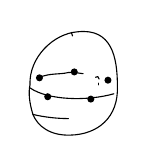
\begin{tikzpicture}[scale=.75,line cap=round,line join=round]
\draw (-.73,-.03) .. controls (-.75,.43) and (-.34,.84) .. (.08,.87)
 .. controls (.65,.93) and (.75,.45) .. (.75,-.05)
 .. controls (.77,-.58) and (.42,-.87) .. (-.05,-.88)
 .. controls (-.39,-.89) and (-.60,-.73) .. (-.68,-.53)
 .. controls (-.74,-.34) and (-.76,-.16) .. (-.73,-.03);
\draw (-.73,-.08) .. controls (-.43,-.29) and (.23,-.31) .. (.69,-.18);
\draw (-.60,.09) .. controls (-.36,.18) and (-.25,.14) .. (-.08,.18)
 .. controls (.01,.19) and (.09,.17) .. (.17,.16);
\draw (.38,.10)--(.42,.11)--(.44,.07);
\draw (.43,0)--(.43,-.03);
\draw (.59,.07)--(.61,.02);
\foreach \x/\y in {-.57/.09,.02/.19,.59/.05,-.43/-.23,.30/-.27}
 {\fill (\x,\y) circle(1.7pt);}
\draw (-.68,-.53) .. controls (-.47,-.58) and (-.25,-.60) .. (-.08,-.60);
\draw (-.03,.86)--(-.01,.80);
\end{tikzpicture}}

\textcircled{2} \(\nu=4\) alors \deleted{\(K=\operatorname{Card}I^g=1\)} \inserted{\(K^g=\{P\}\)}, et \(I\setminus\{P\}\) est une orbite. OPS que c’est \(\mu_4\), sur lequel \(\mu_4\) opère, et \(P\) est un pôle : \(\unsure{\infty|0}\). Le groupe total des autom est \(\mathbb Z/4\mathbb Z\simeq\mu_4(k)\).

La catégorie de ces configurations est équivalente à celle des carrés orientés.

\margin{``pyramide carrée''}
\figure{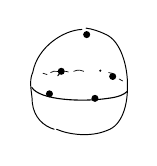
\begin{tikzpicture}[x=.0075cm,y=-.00818cm,line cap=round,line join=round]
\draw[line width=.35pt] (102,14)
 .. controls (71,15) and (27,41) .. (19,80)
 .. controls (11,96) and (18,112) .. (18,128)
 .. controls (21,151) and (37,164) .. (55,169);
\draw[line width=.35pt] (59,169)
 .. controls (79,177) and (115,182) .. (144,171)
 .. controls (171,163) and (179,130) .. (179,104)
 .. controls (180,70) and (167,32) .. (143,22)
 .. controls (132,17) and (119,13) .. (109,12);
\draw[line width=.4pt] (17,104)
 .. controls (31,124) and (102,127) .. (146,121)
 .. controls (163,119) and (172,116) .. (179,110);
\draw[line width=.25pt] (36,82) -- (43,84);
\draw[line width=.25pt] (49,81)
 .. controls (56,76) and (62,82) .. (69,78);
\draw[line width=.25pt] (74,79) -- (79,80);
\draw[line width=.25pt] (88,79)
 .. controls (96,76) and (101,77) .. (105,79);
\draw[line width=.25pt] (147,81) -- (153,82);
\draw[line width=.25pt] (165,91) -- (171,94);
\draw[line width=.35pt] (67,79)--(61,86);
\fill (133,78) circle[radius=.425pt];
\fill (110,22) circle[radius=1.275pt];
\fill (67,79) circle[radius=1.275pt];
\fill (154,87) circle[radius=1.275pt];
\fill (47,114) circle[radius=1.275pt];
\fill (124,121) circle[radius=1.275pt];
\end{tikzpicture}}

\textcircled{3} \(\nu=3\), Alors \deleted{\(\unsure{\Sigma|K}_{\unsure{2}}\)} \(\operatorname{Card}K^g=2\), \inserted{donc \(K^g=\Sigma^g\),} et \(I\setminus K^g\) \inserted{\(=J\)} est une orbite,
\deleted{Le groupe \unsure{total est|des auto}}
\inserted{qu’on peut supposer \(\mu_3\).} La catégorie de ces configurations est équivalente : celle des triangles combinatoires i.e. celle \(\mathrm{Ens}(3)\) des ens \(J\) de Card \(3\).

A \(J\) on associe \(\Sigma_J\unsure{\deleted{\Sigma}|\deleted{g}\Omega|\deleted{G}\Omega}\) avec \(J\cup P_J\) (\(P_J\subset\Sigma_J^{\unsure{g}}\) ens des deux pôles de \(\Sigma_J\) pour corr. \(1\)-\(1\) avec l’ens \(\omega(\unsure{I|J})\) des or. de \(J\), si \(\unsure{k|K}=\mathbb C\)). Groupe des autom. est \(\mathbb D_3\).

\margin{\unsure{Partition|Une partition} \(2\) et \(3\) (par ordre de richesse en symétries)}
\margin{``bitétraèdre''}
\figure{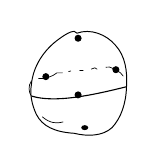
\begin{tikzpicture}[x=.00706cm,y=-.0080cm,line cap=round,line join=round]
\draw[line width=.35pt] (104,16)
 .. controls (128,8) and (157,18) .. (173,35)
 .. controls (191,52) and (195,77) .. (193,102)
 .. controls (192,128) and (183,151) .. (167,166)
 .. controls (150,180) and (122,180) .. (99,175)
 .. controls (64,173) and (42,164) .. (31,145)
 .. controls (23,130) and (19,113) .. (22,98)
 .. controls (25,68) and (45,42) .. (72,25)
 .. controls (86,16) and (100,9) .. (104,16);
\draw[line width=.4pt] (23,116)
 .. controls (64,127) and (130,115) .. (193,101);
\draw[line width=.25pt] (35,88)
 .. controls (46,89) and (60,85) .. (68,79)
 -- (78,79);
\draw[line width=.25pt] (89,77) -- (93,76);
\draw[line width=.25pt] (109,75) -- (115,75);
\draw[line width=.25pt] (130,73) -- (136,71) -- (140,73);
\draw[line width=.25pt] (156,70)
 .. controls (166,68) and (170,74) .. (174,75)
 .. controls (181,77) and (185,81) .. (187,84);
\draw[line width=.25pt] (42,149)
 .. controls (55,159) and (68,160) .. (79,157);
\draw[line width=.25pt] (22,92)..controls(16,99)and(17,110)..(22,116);
\fill (106,24) circle[radius=1.275pt];
\fill (48,85) circle[radius=1.275pt];
\fill (174,74) circle[radius=1.275pt];
\fill (106,114) circle[radius=1.275pt];
\fill (118,166) ellipse[x radius=1.275pt,y radius=.9pt];
\end{tikzpicture}}
\margin{33}
